% ============================================================= %
%  Template LaTeX pour Quarto — Mémoire CNAM style
% ============================================================= 
\documentclass{article}

\usepackage{color}
\usepackage{fancyvrb}
\newcommand{\VerbBar}{|}
\newcommand{\VERB}{\Verb[commandchars=\\\{\}]}
\DefineVerbatimEnvironment{Highlighting}{Verbatim}{commandchars=\\\{\}}
% Add ',fontsize=\small' for more characters per line
\usepackage{framed}
\definecolor{shadecolor}{RGB}{241,243,245}
\newenvironment{Shaded}{\begin{snugshade}}{\end{snugshade}}
\newcommand{\AlertTok}[1]{\textcolor[rgb]{0.68,0.00,0.00}{#1}}
\newcommand{\AnnotationTok}[1]{\textcolor[rgb]{0.37,0.37,0.37}{#1}}
\newcommand{\AttributeTok}[1]{\textcolor[rgb]{0.40,0.45,0.13}{#1}}
\newcommand{\BaseNTok}[1]{\textcolor[rgb]{0.68,0.00,0.00}{#1}}
\newcommand{\BuiltInTok}[1]{\textcolor[rgb]{0.00,0.23,0.31}{#1}}
\newcommand{\CharTok}[1]{\textcolor[rgb]{0.13,0.47,0.30}{#1}}
\newcommand{\CommentTok}[1]{\textcolor[rgb]{0.37,0.37,0.37}{#1}}
\newcommand{\CommentVarTok}[1]{\textcolor[rgb]{0.37,0.37,0.37}{\textit{#1}}}
\newcommand{\ConstantTok}[1]{\textcolor[rgb]{0.56,0.35,0.01}{#1}}
\newcommand{\ControlFlowTok}[1]{\textcolor[rgb]{0.00,0.23,0.31}{\textbf{#1}}}
\newcommand{\DataTypeTok}[1]{\textcolor[rgb]{0.68,0.00,0.00}{#1}}
\newcommand{\DecValTok}[1]{\textcolor[rgb]{0.68,0.00,0.00}{#1}}
\newcommand{\DocumentationTok}[1]{\textcolor[rgb]{0.37,0.37,0.37}{\textit{#1}}}
\newcommand{\ErrorTok}[1]{\textcolor[rgb]{0.68,0.00,0.00}{#1}}
\newcommand{\ExtensionTok}[1]{\textcolor[rgb]{0.00,0.23,0.31}{#1}}
\newcommand{\FloatTok}[1]{\textcolor[rgb]{0.68,0.00,0.00}{#1}}
\newcommand{\FunctionTok}[1]{\textcolor[rgb]{0.28,0.35,0.67}{#1}}
\newcommand{\ImportTok}[1]{\textcolor[rgb]{0.00,0.46,0.62}{#1}}
\newcommand{\InformationTok}[1]{\textcolor[rgb]{0.37,0.37,0.37}{#1}}
\newcommand{\KeywordTok}[1]{\textcolor[rgb]{0.00,0.23,0.31}{\textbf{#1}}}
\newcommand{\NormalTok}[1]{\textcolor[rgb]{0.00,0.23,0.31}{#1}}
\newcommand{\OperatorTok}[1]{\textcolor[rgb]{0.37,0.37,0.37}{#1}}
\newcommand{\OtherTok}[1]{\textcolor[rgb]{0.00,0.23,0.31}{#1}}
\newcommand{\PreprocessorTok}[1]{\textcolor[rgb]{0.68,0.00,0.00}{#1}}
\newcommand{\RegionMarkerTok}[1]{\textcolor[rgb]{0.00,0.23,0.31}{#1}}
\newcommand{\SpecialCharTok}[1]{\textcolor[rgb]{0.37,0.37,0.37}{#1}}
\newcommand{\SpecialStringTok}[1]{\textcolor[rgb]{0.13,0.47,0.30}{#1}}
\newcommand{\StringTok}[1]{\textcolor[rgb]{0.13,0.47,0.30}{#1}}
\newcommand{\VariableTok}[1]{\textcolor[rgb]{0.07,0.07,0.07}{#1}}
\newcommand{\VerbatimStringTok}[1]{\textcolor[rgb]{0.13,0.47,0.30}{#1}}
\newcommand{\WarningTok}[1]{\textcolor[rgb]{0.37,0.37,0.37}{\textit{#1}}}

% ── Packages essentiels ─────────────────────────────────────── 
\usepackage{geometry}
\geometry{a4paper, top=2.5cm, bottom=2.5cm, left=3cm, right=3cm}

\usepackage{microtype}
\usepackage{lmodern}

% ── Couleurs ───────────────────────────────────────────────── 
\usepackage{xcolor}
\usepackage{colortbl}
\definecolor{cnamred}{RGB}{210, 35, 42}
\definecolor{cnamgray}{RGB}{90, 90, 90}
\definecolor{sectionblue}{RGB}{31, 73, 125}
\definecolor{lightgray}{RGB}{245, 245, 245}
\definecolor{rulegray}{RGB}{180, 180, 180}
\definecolor{shadecolor}{RGB}{248, 248, 248}

% ── Graphiques & mise en page ──────────────────────────────── 
\usepackage{graphicx}

% ── Fix pour les images Quarto (pandocbounded) ─────────────── 
\makeatletter
\def\maxwidth{\ifdim\Gin@nat@width>\linewidth\linewidth\else\Gin@nat@width\fi}
\def\maxheight{\ifdim\Gin@nat@height>\textheight\textheight\else\Gin@nat@height\fi}

\newsavebox\pandoc@box
\newcommand*\pandocbounded[1]{%
  \sbox\pandoc@box{#1}%
  \Gscale@div\@tempa{\textheight}{\dimexpr\ht\pandoc@box+\dp\pandoc@box\relax}%
  \Gscale@div\@tempb{\linewidth}{\wd\pandoc@box}%
  \ifdim\@tempb\p@<\@tempa\p@\let\@tempa\@tempb\fi%
  \ifdim\@tempa\p@<\p@\scalebox{\@tempa}{\usebox\pandoc@box}%
  \else\usebox{\pandoc@box}%
  \fi%
}
\makeatother

\usepackage{tikz}
\usepackage{calc}
\usepackage{tabularx}
\usepackage{booktabs}
\usepackage{array}
\usepackage{multirow}
\usepackage{ragged2e}

% ── Typographie des titres ─────────────────────────────────── 
\usepackage{titlesec}

\titleformat{\section}
  {\color{sectionblue}\large\bfseries}
  {\thesection.}{0.6em}{}
  [{\color{rulegray}\vspace{2pt}{\titlerule[0.4pt]}\vspace{4pt}}]

\titleformat{\subsection}
  {\color{sectionblue}\normalsize\bfseries}
  {\thesubsection}{0.6em}{}

\titleformat{\subsubsection}
  {\color{cnamgray}\normalsize\itshape\bfseries}
  {\thesubsubsection}{0.6em}{}

\titlespacing*{\section}{0pt}{18pt}{8pt}
\titlespacing*{\subsection}{0pt}{14pt}{5pt}
\titlespacing*{\subsubsection}{0pt}{10pt}{4pt}

% ── Table des matières ─────────────────────────────────────── 
\usepackage{tocloft}
\renewcommand{\cftsecfont}{\bfseries\color{sectionblue}}
\renewcommand{\cftsecpagefont}{\bfseries\color{sectionblue}}
\renewcommand{\cftsubsecfont}{\color{cnamgray}}
\renewcommand{\cftsubsecpagefont}{\color{cnamgray}}
\renewcommand{\cftsecleader}{\cftdotfill{\cftdotsep}}
\setlength{\cftbeforesecskip}{4pt}

% ── Hyperliens ─────────────────────────────────────────────── 
\usepackage{hyperref}
\hypersetup{
  colorlinks=true,
  linkcolor=sectionblue,
  urlcolor=cnamred,
  citecolor=cnamgray,
  pdfborder={0 0 0}
}

% ── En-têtes et pieds de page ──────────────────────────────── 
\usepackage{fancyhdr}
\pagestyle{fancy}
\fancyhf{}
\fancyhead[L]{\small\color{cnamgray}\textit{Analyse de données}}
\fancyhead[R]{\small\color{cnamgray}Arsène MBABEH - Raphaël PÉNÉ - Oscar JOSEPH--GENESLAY}
\fancyfoot[C]{\small\color{cnamgray}\thepage}
\renewcommand{\headrulewidth}{0.4pt}
\renewcommand{\footrulewidth}{0pt}

% ── Mathématiques ──────────────────────────────────────────── 
\usepackage{amsmath, amssymb, amsthm}

% ── Bibliographie ──────────────────────────────────────────── 

\usepackage[backend=biber, style=apa]{biblatex}
\addbibresource{Ref.bibtex}

% ── Utilitaires Pandoc / Quarto ────────────────────────────── 
\usepackage{longtable}
\usepackage{float}
\usepackage{caption}
\captionsetup{font=small, labelfont={bf,color=sectionblue}, textfont=it}
\usepackage{subcaption}
\usepackage{framed}
\usepackage{wrapfig}
\usepackage{pdflscape}
\usepackage{threeparttable}
\usepackage{threeparttablex}
\usepackage[normalem]{ulem}
\usepackage{makecell}

% ── Fix bug longtable : Pandoc génère \begin{longtable}[]{} ────
\makeatletter
\@ifundefined{c@none}{\newcounter{none}}{}
\makeatother

\providecommand{\tightlist}{%
  \setlength{\itemsep}{2pt}\setlength{\parskip}{0pt}}

% ── Interligne & paragraphes ───────────────────────────────── 
\usepackage{setspace}
\setstretch{1.15}
\setlength{\parskip}{6pt}
\setlength{\parindent}{0pt}

% ── Fix de sécurité pour le bug TikZ ──────────────────────────
\makeatletter
\def\pgfr@layerlist@globally{}
\makeatother

% ============================================================= %
%  DOCUMENT
% ============================================================= 
\begin{document}

% ── PAGE DE GARDE ──────────────────────────────────────────── 
\begin{titlepage}
\thispagestyle{empty}

\begin{tikzpicture}[remember picture, overlay]
  \node[anchor=north east, xshift=-1.5cm, yshift=-1.2cm]
    at (current page.north east) {%
      
\includegraphics[width=4cm, keepaspectratio]{logo_cnam.jpg}
    };
\end{tikzpicture}

\vspace*{2cm}

\begin{center}
  {\large\bfseries{Le Conservatoire National des Arts et M\'{e}tiers}}\\[0.4cm]
  \textcolor{rulegray}{\rule{10cm}{0.4pt}}\\[0.6cm]
  {\normalsize Rapport sur la reproductibilité d'un article scientifique sur l'analyse des données et les probabilités}\\[0.4cm]
  {\normalsize\bfseries Fouille de donn\'{e}es}\\[0.5cm]
  {\small \textit{30 mai 2026} par}\\[0.5cm]
  {\normalsize\bfseries Arsène MBABEH - Raphaël PÉNÉ - Oscar JOSEPH--GENESLAY}\\[0.4cm]
  {\normalsize Promotion (2025-2026)}\\[0.5cm]
  \textcolor{rulegray}{\rule{10cm}{0.4pt}}\\[1.2cm]
  
  % Remplacement de l'ancien bloc TikZ problématique par une boîte stable :
  \setlength{\fboxsep}{14pt}
  \color{cnamgray}
  \framebox[12cm]{%
    \begin{minipage}{11cm}
      \centering
      \color{black}\textbf{Titre :} \textit{Analyse de donnée et probabilité}
    \end{minipage}
  }
\end{center}

\vfill

\begin{center}
  \textcolor{rulegray}{\rule{10cm}{0.4pt}}\\[0.4cm]
  {\small\color{cnamgray} Ann\'{e}e universitaire 2025-2026}
\end{center}

\end{titlepage}

% ── PAGE TABLE DES MATIÈRES ────────────────────────────────── 
\newpage
\thispagestyle{empty}
\renewcommand{\contentsname}{\color{sectionblue}Table des mati\`{e}res}
{
  \hypersetup{linkcolor=sectionblue}
  \tableofcontents
}
\newpage

% ── CORPS DU DOCUMENT ──────────────────────────────────────── 
\setcounter{page}{1}
\pagestyle{fancy}

\#Package

\begin{Shaded}
\begin{Highlighting}[]
\DocumentationTok{\#\#\# Installation des packages}
\CommentTok{\#install.packages("dplyr")}
\CommentTok{\#install.packages("kableExtra")}
\CommentTok{\#install.packages("stargazer")}
\CommentTok{\#install.packages("ggplot2")}
\CommentTok{\#install.packages("ggthemes")}
\CommentTok{\#install.packages("tidyr")}
\CommentTok{\#install.packages("lubridate")}
\end{Highlighting}
\end{Shaded}

\section{Introduction}\label{introduction}

Ce projet explore différents aspects de la statistique : de la théorie
des lois de probabilité à l'analyse de données réelles (Keno) en
s'inspirant de l'article \autocite{Evans2024}.

\subsection{Probabilités
Théoriques}\label{probabilituxe9s-thuxe9oriques}

\subsubsection{Loi de Poisson}\label{loi-de-poisson}

La loi de Poisson est une loi de probabilité \textbf{discrète} qui
décrit le nombre d'événements se produisant dans un intervalle de temps
ou d'espace fixe.

Si \(X \sim \mathcal{P}(\lambda)\), alors :
\[P(X=x)=\frac{\lambda^x}{x!}e^{-\lambda}, \quad x \in \mathbb{N}\]

\begin{Shaded}
\begin{Highlighting}[]
\NormalTok{x }\OtherTok{\textless{}{-}} \DecValTok{0}\SpecialCharTok{:}\DecValTok{10}
\NormalTok{dx }\OtherTok{\textless{}{-}} \FunctionTok{dpois}\NormalTok{(x, }\AttributeTok{lambda =} \DecValTok{3}\NormalTok{)}

\FunctionTok{plot}\NormalTok{(x, dx, }\AttributeTok{type =} \StringTok{"h"}\NormalTok{, }\AttributeTok{lwd =} \DecValTok{2}\NormalTok{, }\AttributeTok{col =} \StringTok{"steelblue"}\NormalTok{,}
     \AttributeTok{main =} \FunctionTok{expression}\NormalTok{(}\StringTok{"Loi de Poisson ("} \SpecialCharTok{*}\NormalTok{ lambda }\SpecialCharTok{==} \DecValTok{3} \SpecialCharTok{*} \StringTok{")"}\NormalTok{),}
     \AttributeTok{xlab =} \StringTok{"Nombre d\textquotesingle{}événements"}\NormalTok{, }\AttributeTok{ylab =} \StringTok{"Probabilité"}\NormalTok{)}
\FunctionTok{points}\NormalTok{(x, dx, }\AttributeTok{pch =} \DecValTok{16}\NormalTok{, }\AttributeTok{col =} \StringTok{"steelblue"}\NormalTok{)}
\end{Highlighting}
\end{Shaded}

\begin{figure}[H]

\centering{

\pandocbounded{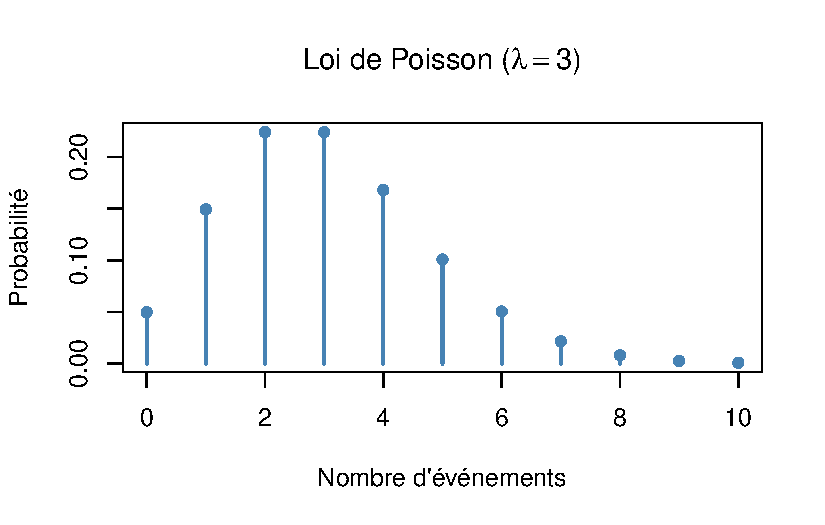
\includegraphics[keepaspectratio]{Programme_Keno_files/figure-pdf/fig-poisson-1.pdf}}

}

\caption{\label{fig-poisson}Distribution de Poisson}

\end{figure}%

\subsubsection{L'esperance
mathématique}\label{lesperance-mathuxe9matique}

L'espérance mathématique, c'est la \textbf{valeur moyenne théorique}
d'une variable aléatoire

\begin{Shaded}
\begin{Highlighting}[]
\CommentTok{\# L\textquotesingle{}espérance c\textquotesingle{}est la somme des x * P(X=x)}
\NormalTok{esperance }\OtherTok{\textless{}{-}} \FunctionTok{sum}\NormalTok{(x }\SpecialCharTok{*}\NormalTok{ dx)}
\FunctionTok{print}\NormalTok{(}\FunctionTok{paste}\NormalTok{(}\StringTok{"Espérance = "}\NormalTok{, }\FunctionTok{round}\NormalTok{(esperance, }\DecValTok{3}\NormalTok{)))}
\end{Highlighting}
\end{Shaded}

\begin{verbatim}
[1] "Espérance =  2.997"
\end{verbatim}

\[ \approx 3\] On peut aussi exécuté le chunck en ligne pour rechercher
le resultat qui est ici : 2.997

\subsubsection{Application Shiny - La Loi
Gamma}\label{application-shiny---la-loi-gamma}

\textbf{Rappel} :

La loi de Gamma est une distribution de probabilité continue qui
modélise des variables aléatoires réelles positives. Elle est utilisée
pour décrire divers phénomènes, tels que la durée de vie d'un système ou
le temps entre des événements.

\begin{Shaded}
\begin{Highlighting}[]
\NormalTok{alpha }\OtherTok{=} \DecValTok{1}
\NormalTok{lambda }\OtherTok{=} \DecValTok{1}
\FunctionTok{curve}\NormalTok{(}\FunctionTok{dgamma}\NormalTok{(x,alpha,lambda), }\DecValTok{0}\NormalTok{, }\DecValTok{10}\NormalTok{)}
\end{Highlighting}
\end{Shaded}

\pandocbounded{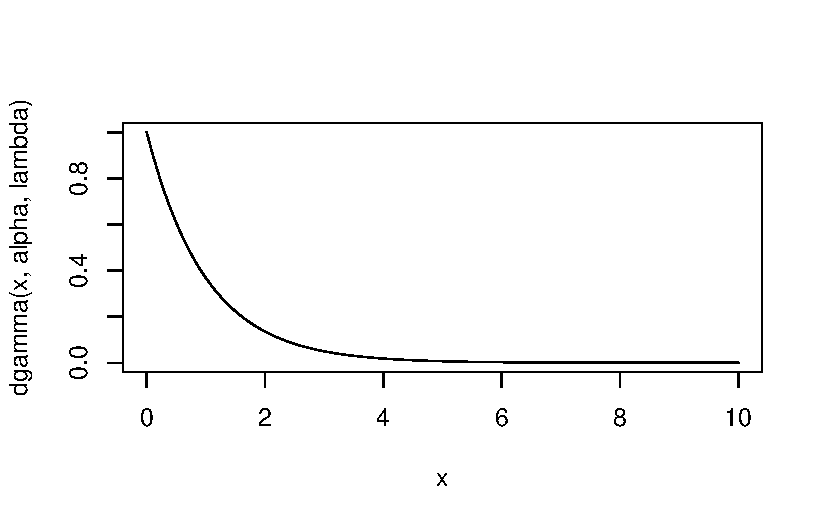
\includegraphics[keepaspectratio]{Programme_Keno_files/figure-pdf/unnamed-chunk-3-1.pdf}}

\subsection{Lancement de l'application
shiny}\label{lancement-de-lapplication-shiny}

https://lapoulefolle64.shinyapps.io/Projet-Killani/

\section{Analyse de Données : data =
``mtcars''}\label{analyse-de-donnuxe9es-data-mtcars}

\subsection{Analyse exploratoire}\label{analyse-exploratoire}

Tout d'abord on commence par afficher les noms des colonnes du dataset
avec la fonction \textbf{\emph{names()}}, puis on crée un résumé
statistique, de tel sorte à obtenir en sortie un tableau présentant des
stats (moyenne et écart-type) des variables mpg et cyl

\begin{Shaded}
\begin{Highlighting}[]
\FunctionTok{library}\NormalTok{(dplyr)}
\FunctionTok{library}\NormalTok{(tidyverse)}
\NormalTok{voiture }\OtherTok{\textless{}{-}}\NormalTok{ mtcars}

\NormalTok{voiture}\SpecialCharTok{|\textgreater{}}\FunctionTok{names}\NormalTok{() }\DocumentationTok{\#\#\# pour voir le nom de chaque colonne}
\end{Highlighting}
\end{Shaded}

\begin{verbatim}
 [1] "mpg"  "cyl"  "disp" "hp"   "drat" "wt"   "qsec" "vs"   "am"   "gear"
[11] "carb"
\end{verbatim}

\begin{Shaded}
\begin{Highlighting}[]
\NormalTok{voiture }\SpecialCharTok{|\textgreater{}} \FunctionTok{select}\NormalTok{(mpg, cyl) }\SpecialCharTok{|\textgreater{}} \FunctionTok{summarise}\NormalTok{(}\AttributeTok{mean\_mpg =} \FunctionTok{mean}\NormalTok{(mpg),}
         \AttributeTok{mean\_cyl =} \FunctionTok{mean}\NormalTok{(cyl), }\AttributeTok{sd\_mpg =} \FunctionTok{sd}\NormalTok{(mpg), }
         \AttributeTok{sd\_cyl =} \FunctionTok{sd}\NormalTok{(cyl) ) }\SpecialCharTok{|\textgreater{}} \FunctionTok{round}\NormalTok{(}\DecValTok{2}\NormalTok{) }\OtherTok{{-}\textgreater{}}\NormalTok{ stat\_desc}
\end{Highlighting}
\end{Shaded}

On transforme les résultats statistiques en une matrice structurée, en
entrant manuellement les valeur (moyenne , écart-type)

\begin{Shaded}
\begin{Highlighting}[]
\FunctionTok{library}\NormalTok{(dplyr)}
\FunctionTok{library}\NormalTok{(kableExtra)}
\end{Highlighting}
\end{Shaded}

\begin{verbatim}

Attaching package: 'kableExtra'
\end{verbatim}

\begin{verbatim}
The following object is masked from 'package:dplyr':

    group_rows
\end{verbatim}

\begin{Shaded}
\begin{Highlighting}[]
\FunctionTok{library}\NormalTok{(tidyverse)}

\NormalTok{stat\_desc }\SpecialCharTok{|\textgreater{}} \FunctionTok{matrix}\NormalTok{(}\FunctionTok{c}\NormalTok{(}\FloatTok{20.02}\NormalTok{, }\FloatTok{6.19}\NormalTok{, }\FloatTok{6.03}\NormalTok{, }\FloatTok{1.79}\NormalTok{), }\AttributeTok{nrow =} \DecValTok{2}\NormalTok{, }
             \AttributeTok{ncol =} \DecValTok{2}\NormalTok{, }\AttributeTok{dimnames =} \FunctionTok{list}\NormalTok{(}\FunctionTok{c}\NormalTok{(}\StringTok{"mean"}\NormalTok{, }\StringTok{"sd"}\NormalTok{),}
             \FunctionTok{c}\NormalTok{(}\StringTok{"mpg"}\NormalTok{, }\StringTok{"cyl"}\NormalTok{))) }\SpecialCharTok{|\textgreater{}} \FunctionTok{kable}\NormalTok{() }\OtherTok{{-}\textgreater{}}\NormalTok{ matrice}

\NormalTok{matrice}
\end{Highlighting}
\end{Shaded}

{\def\LTcaptype{none} % do not increment counter
\begin{longtable}[]{@{}lll@{}}
\toprule\noalign{}
& mpg & cyl \\
\midrule\noalign{}
\endhead
\bottomrule\noalign{}
\endlastfoot
mean & 20.09 & 6.19 \\
sd & 6.03 & 1.79 \\
\end{longtable}
}

\begin{Shaded}
\begin{Highlighting}[]
\FunctionTok{library}\NormalTok{(dplyr)}
\FunctionTok{library}\NormalTok{(kableExtra)}
\FunctionTok{library}\NormalTok{(tidyverse)}

\CommentTok{\# stat desc}
\NormalTok{stat\_desc }\OtherTok{\textless{}{-}}\NormalTok{ mtcars }\SpecialCharTok{|\textgreater{}} 
  \FunctionTok{select}\NormalTok{(mpg, cyl) }\SpecialCharTok{|\textgreater{}} 
  \FunctionTok{summarise}\NormalTok{(}
    \FunctionTok{across}\NormalTok{(}\FunctionTok{everything}\NormalTok{(), }\FunctionTok{list}\NormalTok{(}\AttributeTok{mean =}\NormalTok{ mean, }\AttributeTok{sd =}\NormalTok{ sd))}
\NormalTok{  ) }\SpecialCharTok{|\textgreater{}} 
  \FunctionTok{round}\NormalTok{(}\DecValTok{2}\NormalTok{)}

\CommentTok{\# présentation sous forme de tableau????}
\FunctionTok{kable}\NormalTok{(stat\_desc, }\AttributeTok{caption =} \StringTok{"Moyenne et Écart{-}type (MPG et Cylindres)"}\NormalTok{) }\SpecialCharTok{|\textgreater{}} 
  \FunctionTok{kable\_styling}\NormalTok{(}\AttributeTok{bootstrap\_options =} \StringTok{"striped"}\NormalTok{)}
\end{Highlighting}
\end{Shaded}

\begin{longtable}[t]{rrrr}
\caption{\label{tab:unnamed-chunk-6}Moyenne et Écart-type (MPG et Cylindres)}\\
\toprule
mpg\_mean & mpg\_sd & cyl\_mean & cyl\_sd\\
\midrule
20.09 & 6.03 & 6.19 & 1.79\\
\bottomrule
\end{longtable}

Nous allons ensuite analyser les corrélations entre variables, afin
d'identifier si des relations linéaire existe dans notre jeu de donnée
mtcars

\begin{Shaded}
\begin{Highlighting}[]
\NormalTok{correlation\_matrix }\OtherTok{\textless{}{-}} \FunctionTok{cor}\NormalTok{(mtcars)}
\FunctionTok{heatmap}\NormalTok{(correlation\_matrix)}
\end{Highlighting}
\end{Shaded}

\pandocbounded{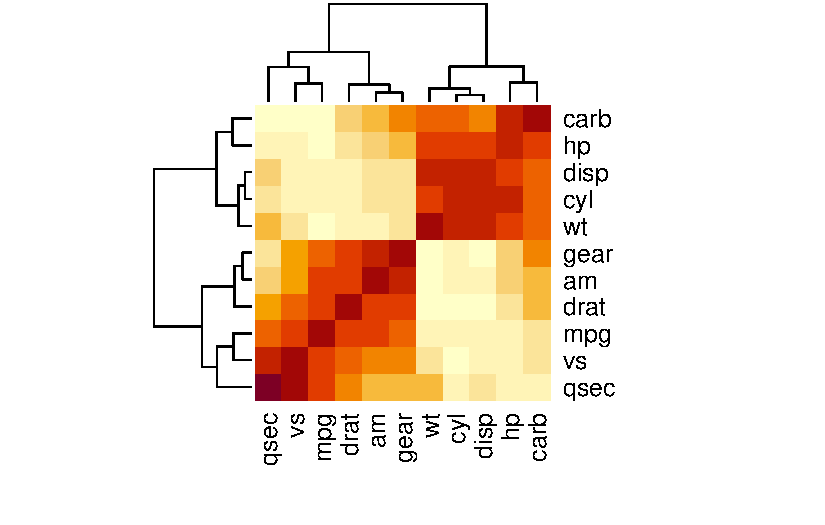
\includegraphics[keepaspectratio]{Programme_Keno_files/figure-pdf/unnamed-chunk-7-1.pdf}}

On constate une corrélation assez faible entre la puissance et la
consommation

\subsection{Regréssion Linéaire}\label{regruxe9ssion-linuxe9aire}

Nous cherchons à expliquer la consommation (mpg) par la puissance (hp),
en utilisant le jeu de donnée mtcars

\begin{Shaded}
\begin{Highlighting}[]
\FunctionTok{library}\NormalTok{(stargazer)}
\FunctionTok{library}\NormalTok{(ggplot2)}
\FunctionTok{library}\NormalTok{(ggthemes)}

\NormalTok{modele }\OtherTok{\textless{}{-}} \FunctionTok{lm}\NormalTok{(mpg }\SpecialCharTok{\textasciitilde{}}\NormalTok{ hp, }\AttributeTok{data =}\NormalTok{ mtcars)}

\CommentTok{\# Tableau de régression }
\CommentTok{\# On commence par extrait les chiffre du summary}
\NormalTok{resultats }\OtherTok{\textless{}{-}} \FunctionTok{coef}\NormalTok{(}\FunctionTok{summary}\NormalTok{(modele))}

\CommentTok{\#puis on met sous forme de tableau}
\NormalTok{knitr}\SpecialCharTok{::}\FunctionTok{kable}\NormalTok{(resultats, }\AttributeTok{digits =} \DecValTok{3}\NormalTok{, }
      \AttributeTok{caption =} \StringTok{"Impact de la puissance (hp) sur}
\StringTok{                  la consommation (mpg)"}\NormalTok{)}
\end{Highlighting}
\end{Shaded}

\begin{longtable}[]{@{}lrrrr@{}}
\caption{Impact de la puissance (hp) sur la consommation
(mpg)}\tabularnewline
\toprule\noalign{}
& Estimate & Std. Error & t value &
Pr(\textgreater\textbar t\textbar) \\
\midrule\noalign{}
\endfirsthead
\toprule\noalign{}
& Estimate & Std. Error & t value &
Pr(\textgreater\textbar t\textbar) \\
\midrule\noalign{}
\endhead
\bottomrule\noalign{}
\endlastfoot
(Intercept) & 30.099 & 1.634 & 18.421 & 0 \\
hp & -0.068 & 0.010 & -6.742 & 0 \\
\end{longtable}

\begin{Shaded}
\begin{Highlighting}[]
\CommentTok{\# Visualisation}
\FunctionTok{ggplot}\NormalTok{(mtcars, }\FunctionTok{aes}\NormalTok{(}\AttributeTok{x =}\NormalTok{ hp, }\AttributeTok{y =}\NormalTok{ mpg)) }\SpecialCharTok{+}
  \FunctionTok{geom\_point}\NormalTok{(}\AttributeTok{col =} \StringTok{"blue"}\NormalTok{, }\AttributeTok{alpha =} \FloatTok{0.6}\NormalTok{) }\SpecialCharTok{+}
  \FunctionTok{geom\_smooth}\NormalTok{(}\AttributeTok{method =} \StringTok{"lm"}\NormalTok{, }\AttributeTok{se =} \ConstantTok{FALSE}\NormalTok{, }\AttributeTok{col =} \StringTok{"red"}\NormalTok{) }\SpecialCharTok{+}
  \FunctionTok{theme\_igray}\NormalTok{() }\SpecialCharTok{+}
  \FunctionTok{labs}\NormalTok{(}\AttributeTok{title =} \StringTok{"Droite de régression"}\NormalTok{, }\AttributeTok{x =} \StringTok{"Puissance (hp)"}\NormalTok{, }\AttributeTok{y =} \StringTok{"Consommation (mpg)"}\NormalTok{)}
\end{Highlighting}
\end{Shaded}

\pandocbounded{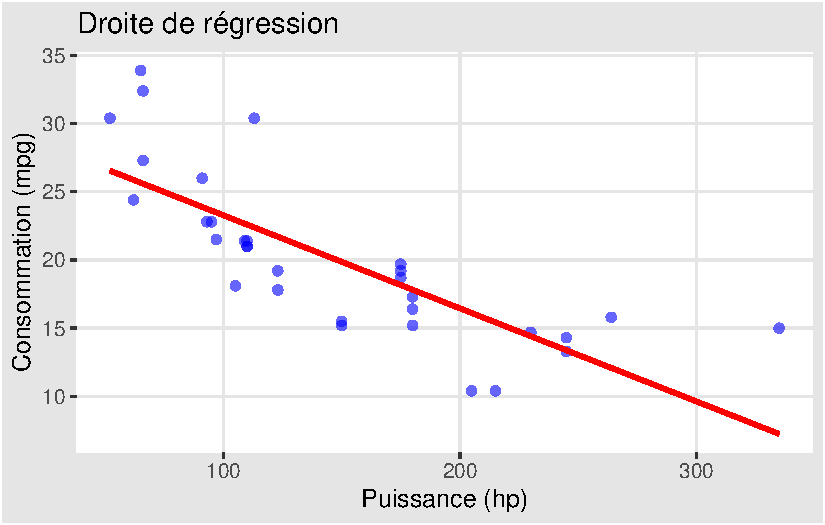
\includegraphics[keepaspectratio]{Programme_Keno_files/figure-pdf/unnamed-chunk-8-1.pdf}}

\subsubsection{Interprétation :}\label{interpruxe9tation}

\textbf{\emph{Le modèle de régression linéaire utilisé est le suivant :
mpg \textasciitilde{} hp, ce qui signifie que la variable ``mpg'' est
expliquée en fonction de la variable hp}}

\begin{itemize}
  \item L’intercept : son estimation est de 30.09, ce qui signifie que lorsque la variable hp est égale à zéro, la variable mpg est estimée à 30.09

  \item Le coefficient de hp : dson estimation est de -0.068, ce qui signifie que pour chaque unité d’augmentation de hp, la variable mpg diminue en moyenne de 0.068 unités
\end{itemize}

Le R\^{}2 est de 0.60, ce qui signifie que le modèle explique environ
60\% de la variance dans la variable mpg, autrement dit la 60\% de la
variabilité de la mpg est expliqué par notre modele

En bref, notre modèle met en évidence le fait que la variable hp a un
effet significatif sur la variable mpg. Pour chaque augmentation d'une
unité de hp, la valeur de mpg va diminuer \[ \approx 0.068\ unité\]
unités

\subsection{Regression en Latex}\label{regression-en-latex}

\begin{Shaded}
\begin{Highlighting}[]
\FunctionTok{library}\NormalTok{(stargazer)}

\NormalTok{modele }\OtherTok{=} \FunctionTok{lm}\NormalTok{(mpg }\SpecialCharTok{\textasciitilde{}}\NormalTok{ hp, }\AttributeTok{data =}\NormalTok{ voiture)}

\DocumentationTok{\#\#\# Pour faire le tableau }
\FunctionTok{stargazer}\NormalTok{(modele,}
          \AttributeTok{type =} \StringTok{"latex"}\NormalTok{,}
          \AttributeTok{title =} \StringTok{"Modèle de régression du mpg expliqué par le hp"}\NormalTok{,}
          \AttributeTok{dep.var.labels =} \StringTok{"mpg"}\NormalTok{,}
          \AttributeTok{covariate.labels =} \StringTok{"hp"}\NormalTok{,}
          \AttributeTok{digits =} \DecValTok{3}\NormalTok{)}
\end{Highlighting}
\end{Shaded}

\% Table created by stargazer v.5.2.3 by Marek Hlavac, Social Policy
Institute. E-mail: marek.hlavac at gmail.com \% Date and time: Thu, May
28, 2026 - 07:49:06 PM

\begin{table}[!htbp] \centering 
  \caption{Modèle de régression du mpg expliqué par le hp} 
  \label{} 
\begin{tabular}{@{\extracolsep{5pt}}lc} 
\\[-1.8ex]\hline 
\hline \\[-1.8ex] 
 & \multicolumn{1}{c}{\textit{Dependent variable:}} \\ 
\cline{2-2} 
\\[-1.8ex] & mpg \\ 
\hline \\[-1.8ex] 
 hp & $-$0.068$^{***}$ \\ 
  & (0.010) \\ 
  & \\ 
 Constant & 30.099$^{***}$ \\ 
  & (1.634) \\ 
  & \\ 
\hline \\[-1.8ex] 
Observations & 32 \\ 
R$^{2}$ & 0.602 \\ 
Adjusted R$^{2}$ & 0.589 \\ 
Residual Std. Error & 3.863 (df = 30) \\ 
F Statistic & 45.460$^{***}$ (df = 1; 30) \\ 
\hline 
\hline \\[-1.8ex] 
\textit{Note:}  & \multicolumn{1}{r}{$^{*}$p$<$0.1; $^{**}$p$<$0.05; $^{***}$p$<$0.01} \\ 
\end{tabular} 
\end{table}

\subsection{Regression avec ggplot}\label{regression-avec-ggplot}

\begin{Shaded}
\begin{Highlighting}[]
\NormalTok{voiture }\SpecialCharTok{|\textgreater{}} \FunctionTok{ggplot}\NormalTok{(}\FunctionTok{aes}\NormalTok{(hp, mpg)) }\SpecialCharTok{+} \FunctionTok{theme\_igray}\NormalTok{() }\SpecialCharTok{+} 
  \FunctionTok{ggtitle}\NormalTok{(}\StringTok{"Consommation en fonction de la puissance"}\NormalTok{) }\SpecialCharTok{+} 
  \FunctionTok{geom\_point}\NormalTok{(}\AttributeTok{col =} \StringTok{"blue"}\NormalTok{) }\SpecialCharTok{+} \FunctionTok{geom\_smooth}\NormalTok{(}\AttributeTok{method =} \StringTok{"lm"}\NormalTok{, }
  \AttributeTok{se =} \ConstantTok{FALSE}\NormalTok{, }\AttributeTok{col =} \StringTok{"red"}\NormalTok{)}
\end{Highlighting}
\end{Shaded}

\pandocbounded{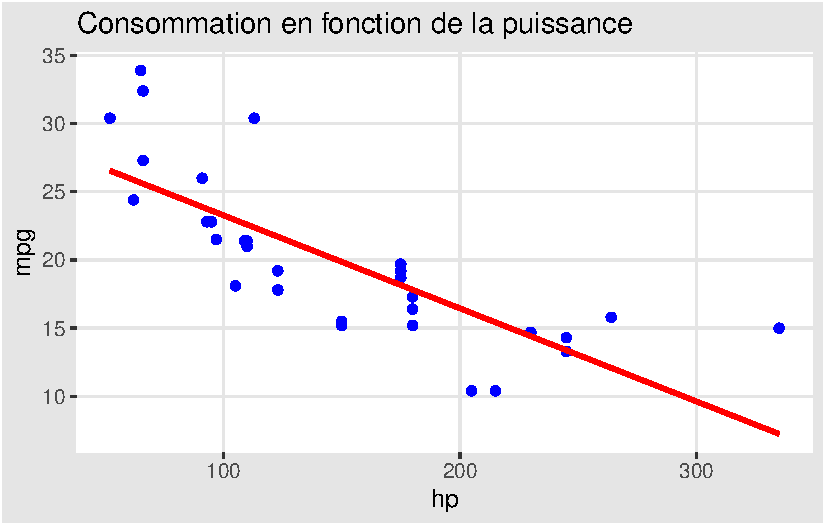
\includegraphics[keepaspectratio]{Programme_Keno_files/figure-pdf/unnamed-chunk-10-1.pdf}}

\section{Travail avec les données
réel}\label{travail-avec-les-donnuxe9es-ruxe9el}

On importe les données historiques du jeu Keno, puis on transforme les
données du format \textbf{large} (c'est à dire une une colonne par
boule) au format \textbf{long} pour faciliter notre analyse

\begin{Shaded}
\begin{Highlighting}[]
\CommentTok{\#| error: false}
\CommentTok{\#| warning: false}
\CommentTok{\#| message: false}

\FunctionTok{library}\NormalTok{(tidyr)}
\FunctionTok{library}\NormalTok{(lubridate)}
\FunctionTok{library}\NormalTok{(tidyr)}
\FunctionTok{library}\NormalTok{(dplyr)}

\NormalTok{df }\OtherTok{=} \FunctionTok{read.csv2}\NormalTok{(}\StringTok{"keno\_202511 6 (1).csv"}\NormalTok{)}

\DocumentationTok{\#\# on supprime des variable }
\NormalTok{df }\OtherTok{=}\NormalTok{ df[,}\SpecialCharTok{{-}}\FunctionTok{c}\NormalTok{(}\DecValTok{1}\NormalTok{, }\DecValTok{3}\NormalTok{,}\DecValTok{20}\NormalTok{,}\DecValTok{21}\NormalTok{,}\DecValTok{22}\NormalTok{,}\DecValTok{23}\NormalTok{)]}

\CommentTok{\# On convertit la date PUIS on bascule au format long}
\NormalTok{df1 }\OtherTok{\textless{}{-}}\NormalTok{ df }\SpecialCharTok{|\textgreater{}}
  \FunctionTok{mutate}\NormalTok{(}\AttributeTok{date\_de\_tirage =} \FunctionTok{dmy}\NormalTok{(date\_de\_tirage)) }\SpecialCharTok{|\textgreater{}}
  \FunctionTok{pivot\_longer}\NormalTok{(}
    \AttributeTok{cols =} \SpecialCharTok{!}\NormalTok{date\_de\_tirage, }
    \AttributeTok{names\_to =} \StringTok{"boule"}\NormalTok{,}
    \AttributeTok{values\_to =} \StringTok{"valeur"}\NormalTok{,}
    \AttributeTok{names\_prefix =} \StringTok{"boule"}
\NormalTok{  )}

\NormalTok{df1}
\end{Highlighting}
\end{Shaded}

\begin{verbatim}
# A tibble: 1,600 x 3
   date_de_tirage boule valeur
   <date>         <chr>  <int>
 1 2026-02-10     1         12
 2 2026-02-10     2         13
 3 2026-02-10     3         17
 4 2026-02-10     4         20
 5 2026-02-10     5         22
 6 2026-02-10     6         23
 7 2026-02-10     7         26
 8 2026-02-10     8         27
 9 2026-02-10     9         39
10 2026-02-10     10        42
# i 1,590 more rows
\end{verbatim}

\begin{Shaded}
\begin{Highlighting}[]
\CommentTok{\# Vérification de la date la plus récente}
\FunctionTok{max}\NormalTok{(df1}\SpecialCharTok{$}\NormalTok{date\_de\_tirage)}
\end{Highlighting}
\end{Shaded}

\begin{verbatim}
[1] "2026-02-10"
\end{verbatim}

\subsubsection{Tableau des fréquences}\label{tableau-des-fruxe9quences}

\begin{Shaded}
\begin{Highlighting}[]
\FunctionTok{library}\NormalTok{(scales)}

\CommentTok{\# Création du tableau des fréquences et pourcentages}
\NormalTok{tableau\_frequences }\OtherTok{\textless{}{-}}\NormalTok{ df1 }\SpecialCharTok{|\textgreater{}} \FunctionTok{group\_by}\NormalTok{(valeur) }\SpecialCharTok{|\textgreater{}} 
  \FunctionTok{summarise}\NormalTok{(}\AttributeTok{Frequence =} \FunctionTok{n}\NormalTok{()) }\SpecialCharTok{|\textgreater{}} 
  \FunctionTok{mutate}\NormalTok{(}\AttributeTok{Pourcentage =} \FunctionTok{percent}\NormalTok{(Frequence }\SpecialCharTok{/} \FunctionTok{sum}\NormalTok{(Frequence), }\AttributeTok{accuracy =} \FloatTok{0.01}\NormalTok{))}

\NormalTok{tableau\_frequences}
\end{Highlighting}
\end{Shaded}

\begin{verbatim}
# A tibble: 56 x 3
   valeur Frequence Pourcentage
    <int>     <int> <chr>      
 1      1        30 1.87%      
 2      2        26 1.62%      
 3      3        28 1.75%      
 4      4        32 2.00%      
 5      5        17 1.06%      
 6      6        21 1.31%      
 7      7        37 2.31%      
 8      8        23 1.44%      
 9      9        33 2.06%      
10     10        30 1.87%      
# i 46 more rows
\end{verbatim}

\subsubsection{La probabilité qu'une boule
sorte}\label{la-probabilituxe9-quune-boule-sorte}

\subsubsection{teste de khi deux}\label{teste-de-khi-deux}

Pour déterminer si les écarts de fréquences observés sont dus au hasard
ou à un biais, nous réalisons un test de conformité à une loi uniforme,
en fait on va chercher à vérifié l'équiprobabilité, c'est à dire qu'on
se pose la question de savoir si toute les boules ont la même
probabilité d'être tiré

Sous l'hypothèse

\begin{itemize}
      \item $H_0$ : Les boules ont toutes la même probabilité de sortir 
      \item $H_1$ : Les boules n'ont pas du tout la même probabilité de sorti
\end{itemize}

NB : Notons que si la p\_value \textless{} alpha : on rejette
l'hypothese null

\begin{Shaded}
\begin{Highlighting}[]
\FunctionTok{chisq.test}\NormalTok{(tableau\_frequences}\SpecialCharTok{$}\NormalTok{Frequence)}
\end{Highlighting}
\end{Shaded}

\begin{verbatim}

    Chi-squared test for given probabilities

data:  tableau_frequences$Frequence
X-squared = 45.14, df = 55, p-value = 0.826
\end{verbatim}

Le test de khi deux sortant une pvalue de 0.82, on conserve l'hypothése
d'équiprobabilité, donc aucune boule n'est statistiquement favorisé

\subsubsection{Simulation de Monté
carlo}\label{simulation-de-montuxe9-carlo}

Afin de renforcer notre conclusion du khi deux, nous simulons 10 000
fois une série de 100 jours de tirages pour observer la distribution du
minimum de fréquence (la boule qui sort le moins souvent).

\begin{Shaded}
\begin{Highlighting}[]
\FunctionTok{set.seed}\NormalTok{(}\DecValTok{123}\NormalTok{)}
\NormalTok{res }\OtherTok{\textless{}{-}} \FunctionTok{c}\NormalTok{()}
\ControlFlowTok{for}\NormalTok{ (i }\ControlFlowTok{in} \DecValTok{1}\SpecialCharTok{:}\DecValTok{10000}\NormalTok{) \{}
  \CommentTok{\# on simule en gros 100 jours de tirages (16 boules parmi 56)}
\NormalTok{  ech }\OtherTok{\textless{}{-}} \FunctionTok{replicate}\NormalTok{(}\DecValTok{100}\NormalTok{, }\FunctionTok{sample}\NormalTok{(}\DecValTok{1}\SpecialCharTok{:}\DecValTok{56}\NormalTok{, }\DecValTok{16}\NormalTok{, }\AttributeTok{replace =} \ConstantTok{FALSE}\NormalTok{))}
\NormalTok{  res }\OtherTok{\textless{}{-}} \FunctionTok{c}\NormalTok{(res, }\FunctionTok{min}\NormalTok{(}\FunctionTok{table}\NormalTok{(ech)))}
\NormalTok{\}}

\FunctionTok{min}\NormalTok{(res)}
\end{Highlighting}
\end{Shaded}

\begin{verbatim}
[1] 9
\end{verbatim}

\begin{Shaded}
\begin{Highlighting}[]
\FunctionTok{library}\NormalTok{(ggplot2)}

\FunctionTok{as\_tibble}\NormalTok{(res) }\SpecialCharTok{|\textgreater{}} \FunctionTok{ggplot}\NormalTok{(}\FunctionTok{aes}\NormalTok{(value)) }\SpecialCharTok{+} 
  \FunctionTok{geom\_bar}\NormalTok{(}\AttributeTok{col =} \StringTok{"red"}\NormalTok{) }\SpecialCharTok{+} 
  \FunctionTok{ggtitle}\NormalTok{(}\StringTok{"Distribution empirique des minimum de fréquence de sortie sur 100 jours"}\NormalTok{)}
\end{Highlighting}
\end{Shaded}

\pandocbounded{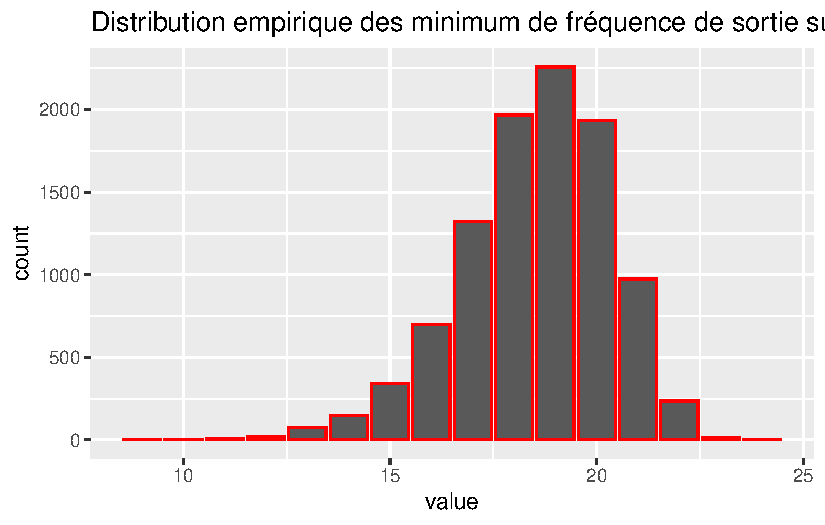
\includegraphics[keepaspectratio]{Programme_Keno_files/figure-pdf/unnamed-chunk-15-1.pdf}}

\begin{Shaded}
\begin{Highlighting}[]
\FunctionTok{as\_tibble}\NormalTok{(res) }\SpecialCharTok{|\textgreater{}} \FunctionTok{filter}\NormalTok{(value }\SpecialCharTok{\textless{}=} \DecValTok{17}\NormalTok{) }\SpecialCharTok{|\textgreater{}} \FunctionTok{summarise}\NormalTok{(}\AttributeTok{Frequence =} \FunctionTok{n}\NormalTok{())}
\end{Highlighting}
\end{Shaded}

\begin{verbatim}
# A tibble: 1 x 1
  Frequence
      <int>
1      2615
\end{verbatim}

p value est forte donc on conserve l'hypothése selon laquelle aucune
boule n'est laisée

% ── BIBLIOGRAPHIE ──────────────────────────────────────────── 
\newpage
\printbibliography

\end{document}
